% Actualización base y acceso a los servidores
\subsection{Actualización base y acceso a los servidores}\label{sec:2_1_actualizacion_acceso}
Las tres VPS son servidores con Ubuntu 24.04.5 LTS contratados con el proveedor Contabo. La administración se realiza de forma remota por SSH con el cliente Termius, usando la cuenta \texttt{root}. Esta sección explica primero cómo se configura ese acceso y después la actualización del sistema y la zona horaria, que es lo primero que se ejecuta al entrar a cada servidor.

\subsubsection{Acceso por SSH como root con Termius}
\paragraph{Cliente utilizado.} Termius es un cliente SSH gráfico para Windows, macOS y Linux que guarda la lista de servidores con sus credenciales, abre cada conexión en una pestaña o en paneles dentro de un mismo espacio de trabajo (\emph{Workspace}) e incluye un explorador SFTP para transferir archivos. Se utiliza en lugar de la terminal del sistema para tener en un solo lugar las tres VPS de la plataforma y trabajar con ellas al mismo tiempo.

\paragraph{Registro de los servidores.} En Termius se crea un \emph{host} por cada VPS desde \textbf{Hosts $\rightarrow$ New host}, con los siguientes datos:

\begin{table}[H]
\centering
\caption{Hosts registrados en Termius}
\small
\begin{tabular}{llccc}
\toprule
\textbf{Label (nombre)} & \textbf{Address} & \textbf{Puerto SSH} & \textbf{Usuario} & \textbf{Autenticación} \\
\midrule
FRONTEND DEFENSORIA & 169.58.62.111 & 22 & root & Contraseña \\
BACKEND DEFENSORIA & 156.67.26.73 & 22 & root & Contraseña \\
BASE DEFENSORIA & 169.58.62.99 & 22 & root & Contraseña \\
\bottomrule
\end{tabular}
\end{table}

\begin{enumerate}
  \item En \textbf{Address} se escribe la IP pública de la VPS.
  \item En \textbf{General} se asigna el nombre con el que aparecerá en la lista (\emph{Label}).
  \item En \textbf{SSH on port} se deja el puerto \texttt{22}.
  \item En \textbf{Credentials} se captura el usuario \texttt{root} y su contraseña. Termius la guarda cifrada en su bóveda (\emph{vault}) personal, por lo que no es necesario escribirla en cada conexión.
  \item Se guarda el host y se repite para las otras dos VPS.
\end{enumerate}

\begin{figure}[H]
\centering
\begin{subfigure}[t]{0.31\textwidth}\centering
  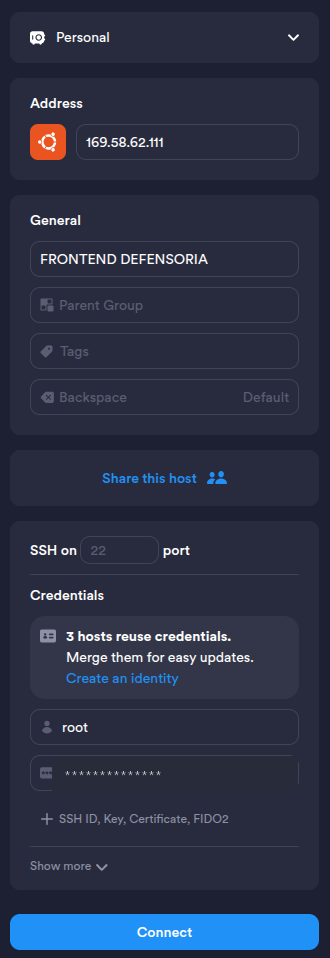
\includegraphics[width=\textwidth]{images/capturas/prep-02-termius-frontend.png}
  \caption{VPS Frontend}
\end{subfigure}\hfill
\begin{subfigure}[t]{0.31\textwidth}\centering
  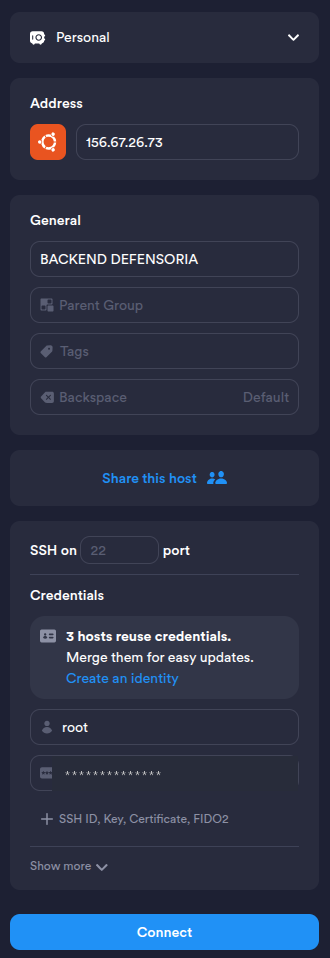
\includegraphics[width=\textwidth]{images/capturas/prep-03-termius-backend.png}
  \caption{VPS Backend}
\end{subfigure}\hfill
\begin{subfigure}[t]{0.31\textwidth}\centering
  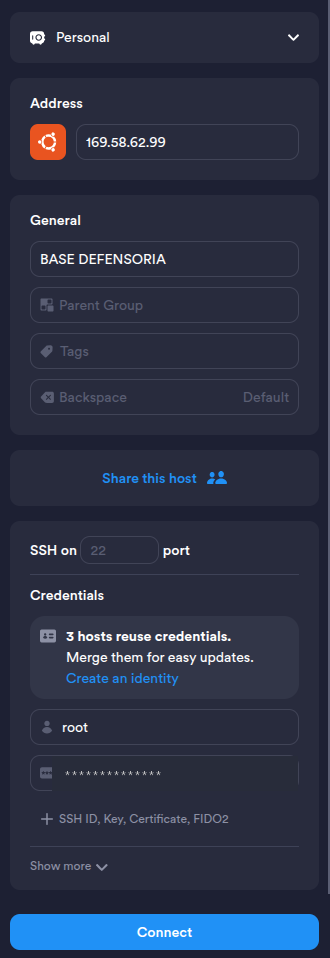
\includegraphics[width=\textwidth]{images/capturas/prep-04-termius-bd.png}
  \caption{VPS Base de Datos}
\end{subfigure}
\caption{Configuración de los tres hosts en Termius (contraseña oculta)}\label{fig:termius-hosts}
\end{figure}

\paragraph{Conexión a las tres VPS.} Al seleccionar un host y pulsar \textbf{Connect}, Termius abre la sesión SSH. En la primera conexión muestra la huella digital (\emph{fingerprint}) de la llave del servidor y pide confirmarla; al aceptarla la registra en \textbf{Known Hosts}. Si en una conexión posterior la huella cambia sin que el servidor se haya reinstalado, se debe rechazar la conexión, porque puede tratarse de un servidor suplantado.

Para la instalación conviene abrir las tres sesiones en un mismo \emph{Workspace}, de modo que las tres VPS quedan visibles a la vez (Figura \ref{fig:prep-05-termius-conexion}). El \emph{prompt} de cada panel muestra el nombre de host del servidor (\texttt{root@vmi3633026}, \texttt{root@vmi3633021}, \texttt{root@vmi3633025}), lo que permite confirmar en qué VPS se está escribiendo antes de ejecutar un comando. La opción \textbf{Broadcast} de Termius envía lo que se escribe a todos los paneles a la vez y sirve para los pasos idénticos en las tres VPS (actualización, zona horaria, instalación de Podman).

\captura{prep-05-termius-conexion}{Sesión SSH como root en las tres VPS dentro de un Workspace de Termius}

\nota{El acceso se hace con usuario \texttt{root} y contraseña, sin llaves SSH. Se recomienda que la contraseña sea larga (16 caracteres o más) y distinta en cada VPS: Termius advierte en la Figura \ref{fig:termius-hosts} que los tres hosts reutilizan las mismas credenciales, de modo que si una se filtra quedan expuestos los tres servidores. Las contraseñas no se escriben en este manual y, al tomar capturas de Termius, el campo de contraseña debe quedar oculto.}

\subsubsection{Actualización del sistema y zona horaria (America/Mexico\_City)}
\paragraph{Actualización de paquetes.} Al conectarse, Ubuntu indica en el mensaje de bienvenida cuántas actualizaciones están pendientes (entre 12 y 14 en la Figura \ref{fig:prep-05-termius-conexion}). En cada VPS se actualiza la lista de paquetes y se instalan:
\begin{lstlisting}
# apt update
# apt upgrade -y
\end{lstlisting}
Si la actualización incluyó un kernel nuevo, Ubuntu crea el archivo \texttt{/var/run/reboot-required}; en ese caso se reinicia la VPS y se vuelve a conectar desde Termius:
\begin{lstlisting}
# [ -f /var/run/reboot-required ] && reboot
\end{lstlisting}

\nota{El mensaje de bienvenida también ofrece actualizar a Ubuntu 26.04 LTS (\texttt{do-release-upgrade}). \textbf{No} se aplica: la plataforma se instaló y probó sobre Ubuntu 24.04 LTS, que sigue recibiendo actualizaciones de seguridad; un cambio de versión mayor se planea por separado.}

\captura{prep-06-apt-upgrade-frontend}{Actualización del sistema en el VPS Frontend}
\captura{prep-07-apt-upgrade-backend}{Actualización del sistema en el VPS Backend}
\captura{prep-08-apt-upgrade-bd}{Actualización del sistema en el VPS Base de Datos}

\paragraph{Zona horaria.} Las VPS vienen con la zona horaria del centro de datos de Contabo en Europa; por eso el mensaje de bienvenida de la Figura \ref{fig:prep-05-termius-conexion} muestra la hora en \texttt{CET}. Se cambian a la hora del centro de México para que las fechas de los registros del sistema, de los logs de los contenedores y de los respaldos coincidan con la hora local de la Defensoría (por ejemplo, el respaldo diario programado a las 4:00 se ejecuta a las 4:00 hora de México y no a media noche):
\begin{lstlisting}
# timedatectl set-timezone America/Mexico_City
# timedatectl
\end{lstlisting}
La salida de \texttt{timedatectl} debe mostrar \texttt{Time zone: America/Mexico\_City (CST, -0600)} y \texttt{System clock synchronized: yes}; esto último indica que el reloj se sincroniza automáticamente por NTP.

\captura{prep-09-zona-horaria-frontend}{Zona horaria America/Mexico\_City en el VPS Frontend}
\captura{prep-10-zona-horaria-backend}{Zona horaria America/Mexico\_City en el VPS Backend}
\captura{prep-11-zona-horaria-bd}{Zona horaria America/Mexico\_City en el VPS Base de Datos}

\nota{La base de datos también trabaja en esta zona horaria: el contenedor \texttt{defensoria-db} se crea con \texttt{TZ=America/Mexico\_City} y el script de inicialización fija la misma zona en \texttt{defensoria\_db} (capítulo \ref{cap:05_despliegue_base_datos}).}
